\documentclass[UTF8,a4paper]{ctexart}
\usepackage[utf8]{inputenc}
\usepackage{amsmath}
\usepackage{pdfpages}
\usepackage{graphicx}
\usepackage{wrapfig}
\usepackage{listings}
\usepackage{color}
\usepackage{alltt}
\usepackage{marvosym}
\usepackage{xcolor}
\lstset{
    numbers=left, 
    numberstyle= \tiny, 
    keywordstyle= \color{ blue!70},
    commentstyle= \color{red!50!green!50!blue!50}, 
    frame=shadowbox, % 阴影效果
    rulesepcolor= \color{ red!20!green!20!blue!20} ,
    escapeinside=``, % 英文分号中可写入中文
    xleftmargin=2em,xrightmargin=2em, aboveskip=1em,
    framexleftmargin=2em
} 
% Style definition file generated by highlight 3.6, http://www.andre-simon.de/ 

% Highlighting theme: Vim Editor 

\newcommand{\hlstd}[1]{\textcolor[rgb]{0,0,0}{#1}}
\newcommand{\hlnum}[1]{\textcolor[rgb]{1,0,0}{#1}}
\newcommand{\hlesc}[1]{\textcolor[rgb]{1,0.13,1}{#1}}
\newcommand{\hlstr}[1]{\textcolor[rgb]{1,0,0}{#1}}
\newcommand{\hlpps}[1]{\textcolor[rgb]{1,0,0}{#1}}
\newcommand{\hlslc}[1]{\textcolor[rgb]{0,0,1}{#1}}
\newcommand{\hlcom}[1]{\textcolor[rgb]{0,0,1}{#1}}
\newcommand{\hlppc}[1]{\textcolor[rgb]{1,0.13,1}{#1}}
\newcommand{\hlopt}[1]{\textcolor[rgb]{0,0,0}{#1}}
\newcommand{\hllin}[1]{\textcolor[rgb]{0,0,1}{#1}}
\newcommand{\hlkwa}[1]{\textcolor[rgb]{0.7,0.41,0.09}{#1}}
\newcommand{\hlkwb}[1]{\textcolor[rgb]{0,1,0}{#1}}
\newcommand{\hlkwc}[1]{\textcolor[rgb]{0.7,0.41,0.09}{#1}}
\newcommand{\hlkwd}[1]{\textcolor[rgb]{0,0,0}{#1}}
\definecolor{bgcolor}{rgb}{1,1,1}


\title{计算机原理第一次实验报告}
\author{张蔚桐\ 2015011493\ 自55}
\begin {document}
\maketitle
\section{实验内容}
\subsection{DEBUG的使用练习}
启动DEBUG, 用A 命令输入实验指导书中程序段,用U 命令对此程序作反汇编,在显示屏上逐行阅读程序,并将机器语言和助记符对照,体会机器码和指令助记符(尤其是指令中的立即数) 之间的对应关系。分别用G、P 及T命令执行此程序,并随时用D 及R 命令检查有关内存单元及寄存器内容。本程序在一块数据区写入了0~F 十六个数,用D 命令可以看到相应数据区内容在程序运行前后的变化,用W 命令将程序存于磁盘,用L 命令将程序取回并反汇编检查程序是否复原。
\subsection{汇编语言上机}
用文本编辑器完成以下汇编程序,保存后采用TASM和LINK先后进行编译和连接。在debug模式下检查程序执行和内存变化情况,发现程序完成了内存段的拷贝和语句输出
\pagecolor{bgcolor}
\noindent
\ttfamily
\hlstd{}\hlslc{;\ Experiment\ 1\ (Tutorial\ Guide,\ p.12)}\hspace*{\fill}\\
\hlstd{}\hspace*{\fill}\\
\hlkwa{NAME\ }\hlstd{prob12\hspace*{\fill}\\
\hspace*{\fill}\\
data\ }\hlkwa{SEGMENT}\hspace*{\fill}\\
\hlstd{\hspace*{\fill}\\
buffer1\ }\hlkwa{DB\ }\hlstd{}\hlnum{0}\hlstd{}\hlopt{,}\hlstd{}\hlnum{1}\hlstd{}\hlopt{,}\hlstd{}\hlnum{2}\hlstd{}\hlopt{,}\hlstd{}\hlnum{3}\hlstd{}\hlopt{,}\hlstd{}\hlnum{4}\hlstd{}\hlopt{,}\hlstd{}\hlnum{5}\hlstd{}\hlopt{,}\hlstd{}\hlnum{6}\hlstd{}\hlopt{,}\hlstd{}\hlnum{7}\hlstd{}\hlopt{,}\hlstd{}\hlnum{8}\hlstd{}\hlopt{,}\hlstd{}\hlnum{9}\hspace*{\fill}\\
\hlstd{\ }\hlkwa{DB\ }\hlstd{}\hlnum{0}\hlstd{}\hlkwb{AH}\hlstd{}\hlopt{,}\hlstd{}\hlnum{0}\hlstd{}\hlkwb{BH}\hlstd{}\hlopt{,}\hlstd{}\hlnum{0}\hlstd{}\hlkwb{CH}\hlstd{}\hlopt{,}\hlstd{}\hlnum{0}\hlstd{}\hlkwb{DH}\hlstd{}\hlopt{,}\hlstd{}\hlnum{0}\hlstd{eh}\hlopt{,}\hlstd{}\hlnum{0}\hlstd{fh}\hlstd{\ \ }\hlstd{}\hspace*{\fill}\\
\hlslc{;just\ a\ count}\hspace*{\fill}\\
\hlstd{buffer2\ }\hlkwa{DB\ }\hlstd{}\hlnum{10h\ }\hlstd{dup}\hlopt{(}\hlstd{}\hlnum{0}\hlstd{}\hlopt{)}\hspace*{\fill}\\
\hlstd{mess\ }\hlkwa{DB\ }\hlstd{}\hlstr{'HAVE\ DONE'}\hlstd{}\hlopt{,}\hlstd{}\hlnum{13}\hlstd{}\hlopt{,}\hlstd{}\hlnum{10}\hlstd{}\hlopt{,}\hlstd{}\hlstr{'\$'}\hlstd{}\hlstd{\ \ \ \ }\hlstd{}\hspace*{\fill}\\
\hlslc{;"HAVE\ DONE$\backslash$r$\backslash$n"}\hspace*{\fill}\\
\hlstd{data\ }\hlkwa{ENDS}\hspace*{\fill}\\
\hlstd{\hspace*{\fill}\\
stack\ }\hlkwa{SEGMENT\ }\hlstd{para\ stack}\hlslc{;\ }\hspace*{\fill}\\
\hlstd{}\hlkwa{DB\ }\hlstd{}\hlnum{100\ }\hlstd{dup}\hlopt{(}\hlstd{?}\hlopt{)}\hspace*{\fill}\\
\hlstd{stack\ }\hlkwa{ENDS}\hlstd{}\hlslc{;}\hspace*{\fill}\\
\hlstd{\hspace*{\fill}\\
code\ }\hlkwa{SEGMENT}\hspace*{\fill}\\
\hlstd{}\hlkwa{ASSUME\ }\hlstd{}\hlkwb{CS}\hlstd{}\hlopt{:}\hlstd{code}\hlopt{,\ }\hlstd{}\hlkwb{DS}\hlstd{}\hlopt{:}\hlstd{data}\hlopt{,\ }\hlstd{}\hlkwb{ES}\hlstd{}\hlopt{:}\hlstd{data}\hlopt{,\ }\hlstd{}\hlkwb{SS}\hlstd{}\hlopt{:}\hlstd{stack}\hspace*{\fill}\\
\hlslc{;Reg\ for\ visit\ data\ block}\hspace*{\fill}\\
\hlstd{}\hspace*{\fill}\\
\hlkwc{START:\ }\hlstd{}\hlkwa{MOV\ }\hlstd{}\hlkwb{AX}\hlstd{}\hlopt{,\ }\hlstd{data}\hspace*{\fill}\\
\hlkwa{MOV\ }\hlstd{}\hlkwb{DS}\hlstd{}\hlopt{,\ }\hlstd{}\hlkwb{AX}\hspace*{\fill}\\
\hlstd{}\hlkwa{MOV\ }\hlstd{}\hlkwb{ES}\hlstd{}\hlopt{,\ }\hlstd{}\hlkwb{AX\ }\hspace*{\fill}\\
\hlstd{}\hlslc{;\ set\ up\ the\ user\ data\ segment}\hspace*{\fill}\\
\hlstd{}\hspace*{\fill}\\
\hlkwa{LEA\ }\hlstd{}\hlkwb{SI}\hlstd{}\hlopt{,\ }\hlstd{buffer1}\hlstd{\ \ }\hlstd{}\hspace*{\fill}\\
\hlslc{;\ maybe\ like\ a\ pointer\ in\ C}\hspace*{\fill}\\
\hlstd{}\hlkwa{LEA\ }\hlstd{}\hlkwb{DI}\hlstd{}\hlopt{,\ }\hlstd{buffer2}\hspace*{\fill}\\
\hlkwa{MOV\ }\hlstd{}\hlkwb{CX}\hlstd{}\hlopt{,\ }\hlstd{}\hlnum{10h}\hspace*{\fill}\\
\hlstd{}\hspace*{\fill}\\
\hlkwc{NEXT:\ }\hlstd{}\hlkwa{MOV\ }\hlstd{}\hlkwb{AL}\hlstd{}\hlopt{,\ {[}}\hlstd{}\hlkwb{SI}\hlstd{}\hlopt{{]}\ }\hspace*{\fill}\\
\hlstd{}\hlslc{;\ load\ the\ {*}si\ (data\ in\ buffer1)}\hspace*{\fill}\\
\hlstd{}\hlkwa{MOV\ }\hlstd{}\hlopt{{[}}\hlstd{}\hlkwb{DI}\hlstd{}\hlopt{{]},\ }\hlstd{}\hlkwb{AL}\hlstd{\ \ }\hlkwb{}\hspace*{\fill}\\
\hlstd{}\hlslc{;\ {*}di=al}\hspace*{\fill}\\
\hlstd{}\hlslc{;\ may\ just\ like\ the\ exchange?}\hspace*{\fill}\\
\hlstd{}\hlkwa{INC\ }\hlstd{}\hlkwb{SI}\hspace*{\fill}\\
\hlstd{}\hlkwa{INC\ }\hlstd{}\hlkwb{DI}\hspace*{\fill}\\
\hlstd{}\hlslc{;++si,++di}\hspace*{\fill}\\
\hlstd{}\hlkwa{DEC\ }\hlstd{}\hlkwb{CX}\hlstd{\ \ \ }\hlkwb{}\hspace*{\fill}\\
\hlstd{}\hlslc{;cx{-}{-}}\hspace*{\fill}\\
\hlstd{}\hspace*{\fill}\\
\hlkwa{JNZ\ }\hlstd{next}\hlstd{\ \ }\hlstd{}\hspace*{\fill}\\
\hlslc{;cpy\ buffer1\ to\ buffer2}\hspace*{\fill}\\
\hlstd{}\hspace*{\fill}\\
\hlkwa{LEA\ }\hlstd{}\hlkwb{DX}\hlstd{}\hlopt{,\ }\hlstd{mess}\hlstd{\ \ }\hlstd{}\hspace*{\fill}\\
\hlslc{;prepare\ for\ output}\hspace*{\fill}\\
\hlstd{}\hlkwa{MOV\ }\hlstd{}\hlkwb{AH}\hlstd{}\hlopt{,\ }\hlstd{}\hlnum{9}\hspace*{\fill}\\
\hlstd{}\hlkwa{INT\ }\hlstd{}\hlnum{21h}\hlstd{\ \ \ }\hlnum{}\hspace*{\fill}\\
\hlstd{}\hlslc{;when\ ah\ ==\ 9\ means\ output\ the\ string\ in\ ds:dx}\hspace*{\fill}\\
\hlstd{\ }\hspace*{\fill}\\
\hlkwa{MOV\ }\hlstd{}\hlkwb{AH}\hlstd{}\hlopt{,\ }\hlstd{}\hlnum{4}\hlstd{}\hlkwb{CH}\hspace*{\fill}\\
\hlstd{}\hlkwa{INT\ }\hlstd{}\hlnum{21h}\hlstd{\ \ \ }\hlnum{}\hspace*{\fill}\\
\hlstd{}\hlslc{;when\ ah\ ==\ 4c\ means\ return\ (al);}\hspace*{\fill}\\
\hlstd{\hspace*{\fill}\\
code\ }\hlkwa{ENDS}\hspace*{\fill}\\
\hlstd{}\hspace*{\fill}\\
\hlkwa{END\ }\hlstd{start}\hspace*{\fill}\\
\mbox{}
\normalfont
\normalsize

\subsection{选做内容}
在上面汇编代码的基础上进行修改,利用循环和累加的操作完成对30H~39H 及41H~46H的写入操作

\pagecolor{bgcolor}
\noindent
\ttfamily
\hlstd{}\hlkwa{NAME\ }\hlstd{prob13\hspace*{\fill}\\
\hspace*{\fill}\\
data\ }\hlkwa{SEGMENT}\hspace*{\fill}\\
\hlstd{buffer1\ }\hlkwa{DB\ }\hlstd{}\hlnum{10h\ }\hlstd{dup}\hlopt{(}\hlstd{}\hlnum{0}\hlstd{}\hlopt{)}\hlstd{\ \ }\hlopt{}\hspace*{\fill}\\
\hlstd{}\hlslc{;calloc(10);}\hspace*{\fill}\\
\hlstd{mess\ }\hlkwa{DB\ }\hlstd{}\hlstr{'HAVE\ DONE'}\hlstd{}\hlopt{,}\hlstd{}\hlnum{13}\hlstd{}\hlopt{,}\hlstd{}\hlnum{10}\hlstd{}\hlopt{,}\hlstd{}\hlstr{'\$'}\hlstd{}\hspace*{\fill}\\
\hlslc{;"HAVE\ DONE$\backslash$r$\backslash$n"}\hspace*{\fill}\\
\hlstd{data\ }\hlkwa{ENDS}\hspace*{\fill}\\
\hlstd{\hspace*{\fill}\\
stack\ }\hlkwa{SEGMENT\ }\hlstd{para\ stack}\hspace*{\fill}\\
\hlkwa{DB\ }\hlstd{}\hlnum{10\ }\hlstd{dup}\hlopt{(}\hlstd{}\hlnum{0}\hlstd{}\hlopt{)}\hlstd{\ \ \ }\hlopt{}\hspace*{\fill}\\
\hlstd{}\hlslc{;when\ using\ DEBUG,\ the\ size\ of\ stack\ }\hspace*{\fill}\\
\hlstd{}\hlslc{;is\ no\ less\ than\ 6}\hspace*{\fill}\\
\hlstd{stack\ }\hlkwa{ENDS}\hspace*{\fill}\\
\hlstd{\hspace*{\fill}\\
code\ }\hlkwa{SEGMENT}\hspace*{\fill}\\
\hlstd{}\hlkwa{ASSUME\ }\hlstd{}\hlkwb{CS}\hlstd{}\hlopt{:}\hlstd{code}\hlopt{,\ }\hlstd{}\hlkwb{DS}\hlstd{}\hlopt{:}\hlstd{data}\hlopt{,\ }\hlstd{}\hlkwb{ES}\hlstd{}\hlopt{:}\hlstd{data}\hlopt{,\ }\hlstd{}\hlkwb{SS}\hlstd{}\hlopt{:}\hlstd{stack}\hspace*{\fill}\\
\hlslc{;Reg\ for\ visit\ data\ block}\hspace*{\fill}\\
\hlstd{}\hspace*{\fill}\\
\hlkwc{START:\ }\hlstd{}\hlkwa{MOV\ }\hlstd{}\hlkwb{AX}\hlstd{}\hlopt{,\ }\hlstd{data}\hspace*{\fill}\\
\hlkwa{MOV\ }\hlstd{}\hlkwb{DS}\hlstd{}\hlopt{,\ }\hlstd{}\hlkwb{AX}\hspace*{\fill}\\
\hlstd{}\hlkwa{MOV\ }\hlstd{}\hlkwb{ES}\hlstd{}\hlopt{,\ }\hlstd{}\hlkwb{AX}\hlstd{\ \ }\hlkwb{}\hspace*{\fill}\\
\hlstd{}\hlslc{;\ set\ up\ the\ user\ data\ segment}\hspace*{\fill}\\
\hlstd{}\hlkwa{LEA\ }\hlstd{}\hlkwb{DI}\hlstd{}\hlopt{,\ }\hlstd{buffer1\ }\hspace*{\fill}\\
\hlslc{;\ a\ pointer\ in\ C}\hspace*{\fill}\\
\hlstd{}\hspace*{\fill}\\
\hlkwa{MOV\ }\hlstd{}\hlkwb{CX}\hlstd{}\hlopt{,\ }\hlstd{}\hlnum{0}\hlstd{}\hlkwb{AH}\hspace*{\fill}\\
\hlstd{}\hlkwa{MOV\ }\hlstd{}\hlkwb{AL}\hlstd{}\hlopt{,}\hlstd{}\hlnum{30h}\hspace*{\fill}\\
\hlstd{}\hlkwc{LOOP1:\ }\hlstd{}\hlkwa{MOV\ }\hlstd{}\hlopt{{[}}\hlstd{}\hlkwb{DI}\hlstd{}\hlopt{{]},\ }\hlstd{}\hlkwb{AL\ }\hspace*{\fill}\\
\hlstd{}\hlslc{;\ {*}di=al}\hspace*{\fill}\\
\hlstd{}\hlkwa{INC\ }\hlstd{}\hlkwb{AL}\hspace*{\fill}\\
\hlstd{}\hlkwa{INC\ }\hlstd{}\hlkwb{DI}\hlstd{\ \ \ }\hlkwb{}\hspace*{\fill}\\
\hlstd{}\hlslc{;++al,++di}\hspace*{\fill}\\
\hlstd{}\hlkwa{LOOP\ }\hlstd{loop1}\hlstd{\ \ }\hlstd{}\hspace*{\fill}\\
\hlslc{;cpy\ al\ to\ buffer2}\hspace*{\fill}\\
\hlstd{}\hspace*{\fill}\\
\hlkwa{MOV\ }\hlstd{}\hlkwb{CX}\hlstd{}\hlopt{,}\hlstd{}\hlnum{06h}\hspace*{\fill}\\
\hlstd{}\hlkwa{MOV\ }\hlstd{}\hlkwb{AL}\hlstd{}\hlopt{,}\hlstd{}\hlnum{41h}\hspace*{\fill}\\
\hlstd{}\hlkwc{LOOP2:\ }\hlstd{}\hlkwa{MOV\ }\hlstd{}\hlopt{{[}}\hlstd{}\hlkwb{DI}\hlstd{}\hlopt{{]},}\hlstd{}\hlkwb{AL}\hspace*{\fill}\\
\hlstd{}\hlkwa{INC\ }\hlstd{}\hlkwb{AL}\hspace*{\fill}\\
\hlstd{}\hlkwa{INC\ }\hlstd{}\hlkwb{DI}\hspace*{\fill}\\
\hlstd{}\hlkwa{LOOP\ }\hlstd{loop2}\hspace*{\fill}\\
\hspace*{\fill}\\
\hlkwa{LEA\ }\hlstd{}\hlkwb{DX}\hlstd{}\hlopt{,\ }\hlstd{mess}\hlstd{\ \ }\hlstd{}\hspace*{\fill}\\
\hlslc{;prepare\ for\ output}\hspace*{\fill}\\
\hlstd{}\hlkwa{MOV\ }\hlstd{}\hlkwb{AH}\hlstd{}\hlopt{,\ }\hlstd{}\hlnum{9}\hspace*{\fill}\\
\hlstd{}\hlkwa{INT\ }\hlstd{}\hlnum{21h}\hlstd{\ \ \ }\hlnum{}\hspace*{\fill}\\
\hlstd{}\hlslc{;when\ ah\ ==\ 9\ means\ output\ the\ string\ in\ ds:d}\hspace*{\fill}\\
\hlstd{}\hlkwa{MOV\ }\hlstd{}\hlkwb{AH}\hlstd{}\hlopt{,\ }\hlstd{}\hlnum{4}\hlstd{}\hlkwb{CH}\hspace*{\fill}\\
\hlstd{}\hlkwa{INT\ }\hlstd{}\hlnum{21h}\hlstd{\ \ \ }\hlnum{}\hspace*{\fill}\\
\hlstd{}\hlslc{;when\ ah\ ==\ 4c\ means\ return\ (al);}\hspace*{\fill}\\
\hlstd{\hspace*{\fill}\\
code\ }\hlkwa{ENDS}\hspace*{\fill}\\
\hlstd{}\hspace*{\fill}\\
\hlkwa{END\ }\hlstd{start}\hspace*{\fill}\\
\mbox{}
\normalfont
\normalsize

\section{程序运行情况}
1.1中的程序0H~FH 依次存放在DS:0200~DS:020F 中。首先将SI、CX、AL 初始化,每次将AL 中的值传到DS:[SI] 指向的内存中,地址SI、内容AL 加1,CX 计数减1。循环10 次后,通过INT 结束程序。

1.2中的程序通过累加和循环完成内存块之间的拷贝工作

1.3中的选做程序通过累加和两段循环的方式完成对内存块的写入工作,和1.2不同的是,采用了LOOP命令进行流程控制
\section{总结}
通过这次实验,我熟悉了DOS环境和DEBUG的相关使用方法,对汇编语言也有了更多的体验和了解。为后续实验做好了准备
\begin{figure}
\centering
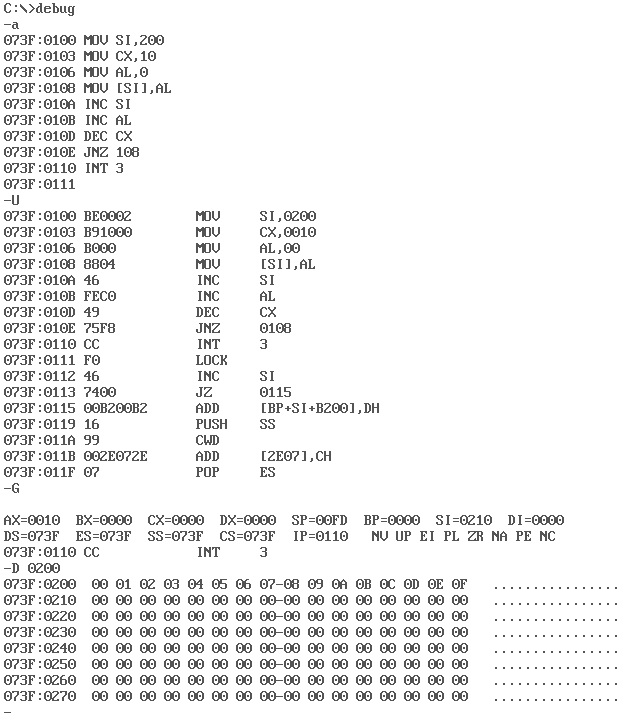
\includegraphics[width=\textwidth]{1-2.jpg}
\caption{1.1运行截图}
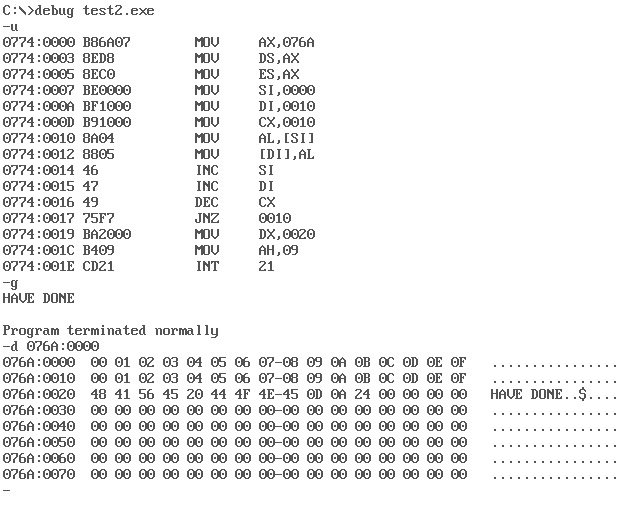
\includegraphics[width=\textwidth]{1-3.jpg}
\caption{1.2运行截图}
\end{figure}
\end{document}